\documentclass[tikz,border=4pt]{standalone}
\usepackage[T1]{fontenc}
\usepackage{lmodern}
\begin{document}
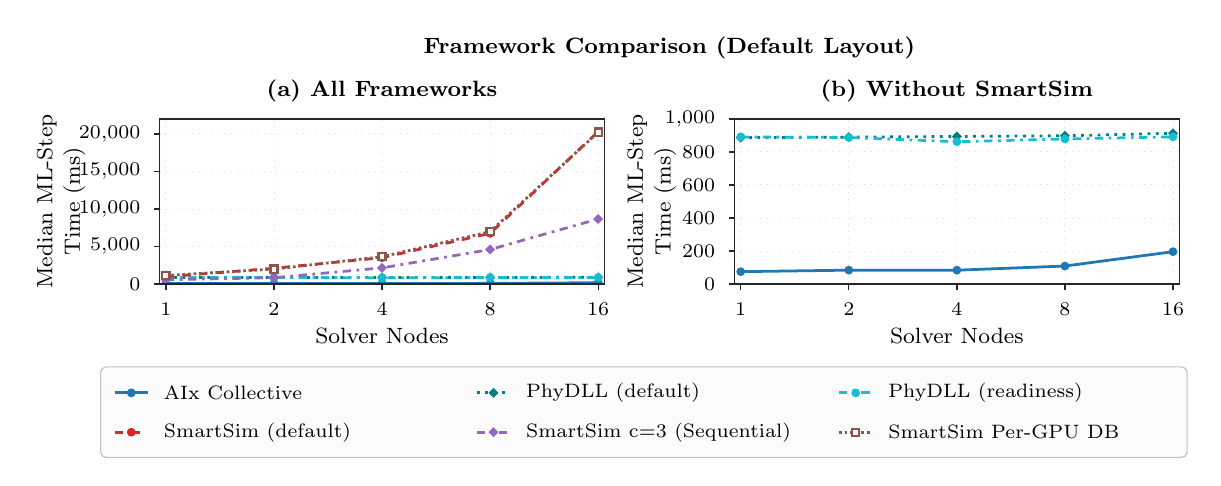
\begin{tikzpicture}[font=\fontsize{8}{10}\selectfont,
axis/.style={black!85,line width=0.5pt},
grid/.style={black!14,line width=0.35pt,dotted},
tick/.style={font=\fontsize{7}{8.5}\selectfont},
title/.style={font=\fontsize{8}{10}\selectfont\bfseries}]
\definecolor{caix_coll}{HTML}{1F77B4}
\definecolor{caix_p2p}{HTML}{FF7F0E}
\definecolor{caix_p2p_fc}{HTML}{2CA02C}
\definecolor{cphydll_default}{HTML}{008080}
\definecolor{cphydll_readiness}{HTML}{17BECF}
\definecolor{csmartsim_c0}{HTML}{D62728}
\definecolor{csmartsim_c3}{HTML}{9467BD}
\definecolor{csmartsim_per_gpu_db}{HTML}{8C564B}
\node[title] at (6.475,3.000) {Framework Comparison (Default Layout)};
\begin{scope}[shift={(0.000,0)}]
\node[title] at (2.825,2.450) {(a) All Frameworks};
\draw[grid] (0,0.0000) -- (5.650,0.0000);
\draw[axis] (0,0.0000) -- (-0.07,0.0000);
\node[tick,anchor=east] at (-0.12,0.0000) {0};
\draw[grid] (0,0.4773) -- (5.650,0.4773);
\draw[axis] (0,0.4773) -- (-0.07,0.4773);
\node[tick,anchor=east] at (-0.12,0.4773) {5,000};
\draw[grid] (0,0.9545) -- (5.650,0.9545);
\draw[axis] (0,0.9545) -- (-0.07,0.9545);
\node[tick,anchor=east] at (-0.12,0.9545) {10,000};
\draw[grid] (0,1.4318) -- (5.650,1.4318);
\draw[axis] (0,1.4318) -- (-0.07,1.4318);
\node[tick,anchor=east] at (-0.12,1.4318) {15,000};
\draw[grid] (0,1.9091) -- (5.650,1.9091);
\draw[axis] (0,1.9091) -- (-0.07,1.9091);
\node[tick,anchor=east] at (-0.12,1.9091) {20,000};
\draw[grid] (0.0800,0) -- (0.0800,2.1);
\draw[axis] (0.0800,0) -- (0.0800,-0.07);
\node[tick,anchor=north] at (0.0800,-0.12) {1};
\draw[grid] (1.4525,0) -- (1.4525,2.1);
\draw[axis] (1.4525,0) -- (1.4525,-0.07);
\node[tick,anchor=north] at (1.4525,-0.12) {2};
\draw[grid] (2.8250,0) -- (2.8250,2.1);
\draw[axis] (2.8250,0) -- (2.8250,-0.07);
\node[tick,anchor=north] at (2.8250,-0.12) {4};
\draw[grid] (4.1975,0) -- (4.1975,2.1);
\draw[axis] (4.1975,0) -- (4.1975,-0.07);
\node[tick,anchor=north] at (4.1975,-0.12) {8};
\draw[grid] (5.5700,0) -- (5.5700,2.1);
\draw[axis] (5.5700,0) -- (5.5700,-0.07);
\node[tick,anchor=north] at (5.5700,-0.12) {16};
\node at (2.825,-0.65) {Solver Nodes};
\node[rotate=90,align=center] at (-1.25,1.050) {Median ML-Step\\Time (ms)};
\begin{scope}
\clip (0,0) rectangle (5.65,2.1);
% aix_coll_default: 75.72750, 84.86250, 84.62150, 109.77150, 196.49100 ms
\draw[caix_coll,line width=1pt,solid] (0.0800,0.0072) -- (1.4525,0.0081) -- (2.8250,0.0081) -- (4.1975,0.0105) -- (5.5700,0.0188);
\fill[caix_coll] (0.0800,0.0072) circle (1.6pt);
\fill[caix_coll] (1.4525,0.0081) circle (1.6pt);
\fill[caix_coll] (2.8250,0.0081) circle (1.6pt);
\fill[caix_coll] (4.1975,0.0105) circle (1.6pt);
\fill[caix_coll] (5.5700,0.0188) circle (1.6pt);
% phydll_default: 885.98850, 889.43200, 893.32200, 897.58450, 912.67050 ms
\draw[cphydll_default,line width=1pt,dotted] (0.0800,0.0846) -- (1.4525,0.0849) -- (2.8250,0.0853) -- (4.1975,0.0857) -- (5.5700,0.0871);
\fill[cphydll_default] (0.0800,0.0846) +(-1.8pt,0) -- +(0,1.8pt) -- +(1.8pt,0) -- +(0,-1.8pt) -- cycle;
\fill[cphydll_default] (1.4525,0.0849) +(-1.8pt,0) -- +(0,1.8pt) -- +(1.8pt,0) -- +(0,-1.8pt) -- cycle;
\fill[cphydll_default] (2.8250,0.0853) +(-1.8pt,0) -- +(0,1.8pt) -- +(1.8pt,0) -- +(0,-1.8pt) -- cycle;
\fill[cphydll_default] (4.1975,0.0857) +(-1.8pt,0) -- +(0,1.8pt) -- +(1.8pt,0) -- +(0,-1.8pt) -- cycle;
\fill[cphydll_default] (5.5700,0.0871) +(-1.8pt,0) -- +(0,1.8pt) -- +(1.8pt,0) -- +(0,-1.8pt) -- cycle;
% phydll_readiness: 890.99000, 887.02450, 861.51300, 878.20250, 891.21550 ms
\draw[cphydll_readiness,line width=1pt,dashdotted] (0.0800,0.0850) -- (1.4525,0.0847) -- (2.8250,0.0822) -- (4.1975,0.0838) -- (5.5700,0.0851);
\fill[cphydll_readiness] (0.0800,0.0850) circle (1.6pt);
\fill[cphydll_readiness] (1.4525,0.0847) circle (1.6pt);
\fill[cphydll_readiness] (2.8250,0.0822) circle (1.6pt);
\fill[cphydll_readiness] (4.1975,0.0838) circle (1.6pt);
\fill[cphydll_readiness] (5.5700,0.0851) circle (1.6pt);
% smartsim_c0: 983.53600, 2121.12000, 3522.41000, 6761.40000, 20301.45000 ms
\draw[csmartsim_c0,line width=1pt,dashed] (0.0800,0.0939) -- (1.4525,0.2025) -- (2.8250,0.3362) -- (4.1975,0.6454) -- (5.5700,1.9379);
\fill[csmartsim_c0] (0.0800,0.0939) circle (1.6pt);
\fill[csmartsim_c0] (1.4525,0.2025) circle (1.6pt);
\fill[csmartsim_c0] (2.8250,0.3362) circle (1.6pt);
\fill[csmartsim_c0] (4.1975,0.6454) circle (1.6pt);
\fill[csmartsim_c0] (5.5700,1.9379) circle (1.6pt);
% smartsim_c3: 591.48500, 863.04150, 2167.70000, 4610.07000, 8673.93000 ms
\draw[csmartsim_c3,line width=1pt,dashdotted] (0.0800,0.0565) -- (1.4525,0.0824) -- (2.8250,0.2069) -- (4.1975,0.4401) -- (5.5700,0.8280);
\fill[csmartsim_c3] (0.0800,0.0565) +(-1.8pt,0) -- +(0,1.8pt) -- +(1.8pt,0) -- +(0,-1.8pt) -- cycle;
\fill[csmartsim_c3] (1.4525,0.0824) +(-1.8pt,0) -- +(0,1.8pt) -- +(1.8pt,0) -- +(0,-1.8pt) -- cycle;
\fill[csmartsim_c3] (2.8250,0.2069) +(-1.8pt,0) -- +(0,1.8pt) -- +(1.8pt,0) -- +(0,-1.8pt) -- cycle;
\fill[csmartsim_c3] (4.1975,0.4401) +(-1.8pt,0) -- +(0,1.8pt) -- +(1.8pt,0) -- +(0,-1.8pt) -- cycle;
\fill[csmartsim_c3] (5.5700,0.8280) +(-1.8pt,0) -- +(0,1.8pt) -- +(1.8pt,0) -- +(0,-1.8pt) -- cycle;
% smartsim_per_gpu_db: 1156.71000, 2006.82000, 3649.60500, 6985.30500, 20228.40000 ms
\draw[csmartsim_per_gpu_db,line width=1pt,densely dotted] (0.0800,0.1104) -- (1.4525,0.1916) -- (2.8250,0.3484) -- (4.1975,0.6668) -- (5.5700,1.9309);
\draw[csmartsim_per_gpu_db,fill=white,line width=0.8pt] (0.0350,0.0654) rectangle (0.1250,0.1554);
\draw[csmartsim_per_gpu_db,fill=white,line width=0.8pt] (1.4075,0.1466) rectangle (1.4975,0.2366);
\draw[csmartsim_per_gpu_db,fill=white,line width=0.8pt] (2.7800,0.3034) rectangle (2.8700,0.3934);
\draw[csmartsim_per_gpu_db,fill=white,line width=0.8pt] (4.1525,0.6218) rectangle (4.2425,0.7118);
\draw[csmartsim_per_gpu_db,fill=white,line width=0.8pt] (5.5250,1.8859) rectangle (5.6150,1.9759);
\end{scope}
\draw[axis] (0,0) rectangle (5.65,2.1);
\end{scope}
\begin{scope}[shift={(7.300,0)}]
\node[title] at (2.825,2.450) {(b) Without SmartSim};
\draw[grid] (0,0.0000) -- (5.650,0.0000);
\draw[axis] (0,0.0000) -- (-0.07,0.0000);
\node[tick,anchor=east] at (-0.12,0.0000) {0};
\draw[grid] (0,0.4200) -- (5.650,0.4200);
\draw[axis] (0,0.4200) -- (-0.07,0.4200);
\node[tick,anchor=east] at (-0.12,0.4200) {200};
\draw[grid] (0,0.8400) -- (5.650,0.8400);
\draw[axis] (0,0.8400) -- (-0.07,0.8400);
\node[tick,anchor=east] at (-0.12,0.8400) {400};
\draw[grid] (0,1.2600) -- (5.650,1.2600);
\draw[axis] (0,1.2600) -- (-0.07,1.2600);
\node[tick,anchor=east] at (-0.12,1.2600) {600};
\draw[grid] (0,1.6800) -- (5.650,1.6800);
\draw[axis] (0,1.6800) -- (-0.07,1.6800);
\node[tick,anchor=east] at (-0.12,1.6800) {800};
\draw[grid] (0,2.1000) -- (5.650,2.1000);
\draw[axis] (0,2.1000) -- (-0.07,2.1000);
\node[tick,anchor=east] at (-0.12,2.1000) {1,000};
\draw[grid] (0.0800,0) -- (0.0800,2.1);
\draw[axis] (0.0800,0) -- (0.0800,-0.07);
\node[tick,anchor=north] at (0.0800,-0.12) {1};
\draw[grid] (1.4525,0) -- (1.4525,2.1);
\draw[axis] (1.4525,0) -- (1.4525,-0.07);
\node[tick,anchor=north] at (1.4525,-0.12) {2};
\draw[grid] (2.8250,0) -- (2.8250,2.1);
\draw[axis] (2.8250,0) -- (2.8250,-0.07);
\node[tick,anchor=north] at (2.8250,-0.12) {4};
\draw[grid] (4.1975,0) -- (4.1975,2.1);
\draw[axis] (4.1975,0) -- (4.1975,-0.07);
\node[tick,anchor=north] at (4.1975,-0.12) {8};
\draw[grid] (5.5700,0) -- (5.5700,2.1);
\draw[axis] (5.5700,0) -- (5.5700,-0.07);
\node[tick,anchor=north] at (5.5700,-0.12) {16};
\node at (2.825,-0.65) {Solver Nodes};
\node[rotate=90,align=center] at (-1.05,1.050) {Median ML-Step\\Time (ms)};
\begin{scope}
\clip (0,0) rectangle (5.65,2.1);
% aix_coll_default: 75.72750, 84.86250, 84.62150, 109.77150, 196.49100 ms
\draw[caix_coll,line width=1pt,solid] (0.0800,0.1590) -- (1.4525,0.1782) -- (2.8250,0.1777) -- (4.1975,0.2305) -- (5.5700,0.4126);
\fill[caix_coll] (0.0800,0.1590) circle (1.6pt);
\fill[caix_coll] (1.4525,0.1782) circle (1.6pt);
\fill[caix_coll] (2.8250,0.1777) circle (1.6pt);
\fill[caix_coll] (4.1975,0.2305) circle (1.6pt);
\fill[caix_coll] (5.5700,0.4126) circle (1.6pt);
% phydll_default: 885.98850, 889.43200, 893.32200, 897.58450, 912.67050 ms
\draw[cphydll_default,line width=1pt,dotted] (0.0800,1.8606) -- (1.4525,1.8678) -- (2.8250,1.8760) -- (4.1975,1.8849) -- (5.5700,1.9166);
\fill[cphydll_default] (0.0800,1.8606) +(-1.8pt,0) -- +(0,1.8pt) -- +(1.8pt,0) -- +(0,-1.8pt) -- cycle;
\fill[cphydll_default] (1.4525,1.8678) +(-1.8pt,0) -- +(0,1.8pt) -- +(1.8pt,0) -- +(0,-1.8pt) -- cycle;
\fill[cphydll_default] (2.8250,1.8760) +(-1.8pt,0) -- +(0,1.8pt) -- +(1.8pt,0) -- +(0,-1.8pt) -- cycle;
\fill[cphydll_default] (4.1975,1.8849) +(-1.8pt,0) -- +(0,1.8pt) -- +(1.8pt,0) -- +(0,-1.8pt) -- cycle;
\fill[cphydll_default] (5.5700,1.9166) +(-1.8pt,0) -- +(0,1.8pt) -- +(1.8pt,0) -- +(0,-1.8pt) -- cycle;
% phydll_readiness: 890.99000, 887.02450, 861.51300, 878.20250, 891.21550 ms
\draw[cphydll_readiness,line width=1pt,dashdotted] (0.0800,1.8711) -- (1.4525,1.8628) -- (2.8250,1.8092) -- (4.1975,1.8442) -- (5.5700,1.8716);
\fill[cphydll_readiness] (0.0800,1.8711) circle (1.6pt);
\fill[cphydll_readiness] (1.4525,1.8628) circle (1.6pt);
\fill[cphydll_readiness] (2.8250,1.8092) circle (1.6pt);
\fill[cphydll_readiness] (4.1975,1.8442) circle (1.6pt);
\fill[cphydll_readiness] (5.5700,1.8716) circle (1.6pt);
\end{scope}
\draw[axis] (0,0) rectangle (5.65,2.1);
\end{scope}
\draw[black!25,fill=gray!3,rounded corners=2pt] (-0.75,-2.1999999999999997) rectangle (13.050,-1.05);
\draw[caix_coll,line width=1pt,solid] (-0.570,-1.380) -- (-0.150,-1.380);
\fill[caix_coll] (-0.3600,-1.3800) circle (1.6pt);
\node[anchor=west,font=\fontsize{7}{8.5}\selectfont] at (-0.070,-1.380) {AIx Collective};
\draw[cphydll_default,line width=1pt,dotted] (4.030,-1.380) -- (4.450,-1.380);
\fill[cphydll_default] (4.2400,-1.3800) +(-1.8pt,0) -- +(0,1.8pt) -- +(1.8pt,0) -- +(0,-1.8pt) -- cycle;
\node[anchor=west,font=\fontsize{7}{8.5}\selectfont] at (4.530,-1.380) {PhyDLL (default)};
\draw[cphydll_readiness,line width=1pt,dashdotted] (8.630,-1.380) -- (9.050,-1.380);
\fill[cphydll_readiness] (8.8400,-1.3800) circle (1.6pt);
\node[anchor=west,font=\fontsize{7}{8.5}\selectfont] at (9.130,-1.380) {PhyDLL (readiness)};
\draw[csmartsim_c0,line width=1pt,dashed] (-0.570,-1.880) -- (-0.150,-1.880);
\fill[csmartsim_c0] (-0.3600,-1.8800) circle (1.6pt);
\node[anchor=west,font=\fontsize{7}{8.5}\selectfont] at (-0.070,-1.880) {SmartSim (default)};
\draw[csmartsim_c3,line width=1pt,dashdotted] (4.030,-1.880) -- (4.450,-1.880);
\fill[csmartsim_c3] (4.2400,-1.8800) +(-1.8pt,0) -- +(0,1.8pt) -- +(1.8pt,0) -- +(0,-1.8pt) -- cycle;
\node[anchor=west,font=\fontsize{7}{8.5}\selectfont] at (4.530,-1.880) {SmartSim c=3 (Sequential)};
\draw[csmartsim_per_gpu_db,line width=1pt,densely dotted] (8.630,-1.880) -- (9.050,-1.880);
\draw[csmartsim_per_gpu_db,fill=white,line width=0.8pt] (8.7950,-1.9250) rectangle (8.8850,-1.8350);
\node[anchor=west,font=\fontsize{7}{8.5}\selectfont] at (9.130,-1.880) {SmartSim Per-GPU DB};
\end{tikzpicture}
\end{document}
